\documentclass[a4paper,10pt]{article}

\usepackage[brazilian]{babel}
\usepackage[utf8]{inputenc}
\usepackage[T1]{fontenc}
\usepackage{titlesec}
\usepackage{graphicx}
\usepackage{mathtools}
\usepackage{amsthm}
\usepackage[top=1.0in,bottom=1.0in]{geometry}
\usepackage{hyperref}
\usepackage[singlelinecheck=false]{caption}
\usepackage[backend=biber,url=true,doi=true,eprint=false]{biblatex}
\usepackage{enumitem}
\usepackage[x11names, rgb]{xcolor}
\usepackage{tikz}
\usetikzlibrary{snakes,arrows,shapes}

\addbibresource{../common/references.bib}

\newcommand\blfootnote[1]{%
  \begingroup
  \renewcommand\thefootnote{}\footnote{#1}%
  \addtocounter{footnote}{-1}%
  \endgroup
}

\newcommand\defeq{\mathrel{\overset{\makebox[0pt]{\mbox{\normalfont\tiny\sffamily def}}}{=}}}

\titleformat{\section}
  {\normalfont\scshape\bfseries}{\thesection}{1em}{}
\titleformat{\subsection}
  {\normalfont\scshape\bfseries}{\thesubsection}{1em}{}
\titleformat{\paragraph}
  {\normalfont}{\theparagraph}{1em}{}
\titleformat{\subparagraph}
  {\normalfont}{\thesubparagraph}{1em}{}

\captionsetup[table]{labelsep=space}

\theoremstyle{plain}

\newtheorem{spn-def}{Definição}
\newtheorem{spn-thm}{Teorema}

\title{\textbf{Uma Introdução a Sum-Product Networks}}

\begin{document}
\date{}
\author{}
\vspace*{-40pt}
{\let\newpage\relax\maketitle}

Relatório semana 9 - MAC0215 (Atividade Curricular em Pesquisa)

Aluno: Renato Lui Geh (Bacharelado em Ciência da Computação)

Orientador: Denis Deratani Mauá

\section{Atividades realizadas na semana}

\paragraph{
  Durante a semana foram lidos as seguintes partes dos papers abaixo:
}

\begin{itemize}
  \item \textit{Learning the Structure of Sum-Product Networks}, [R. Gens, P. Domingos]
    \cite{gens-domingos}
    \begin{itemize}
      \item Introduction
      \item Sum-Product Networks
    \end{itemize}
  \item \textit{Sum-Product Networks: A New Deep Architecture}, [H. Poon, P. Domingos]
    \cite{poon-domingos}
    \begin{itemize}
      \item Introduction
      \item Sum-Product Networks
      \item Sum-Product Networks and other models
    \end{itemize}
\end{itemize}

\section{Definição das atividades}

\paragraph{
  Os tópicos mencionados na seção anterior referem-se à definição de uma Sum-Product Network e
  citam algumas semelhanças com outros modelos probabilísticos assim como suas diferenças.
}

\paragraph{
  Neste relatório vamos definir o que são Sum-Product Networks de uma forma mais didática e vamos
  supor que o leitor tenha conhecimento prévio de todo conteúdo coberto nos relatórios anteriores.
  Após termos definido Sum-Product Networks, vamos ver algumas propriedades e teoremas relacionados
  e em seguida vamos comparar, de forma sucinta, com outros modelos probabilísticos.
}

\paragraph{
  Vamos separar esta seção nos seguintes tópicos:
}

\begin{enumerate}
  \item Introdução
    \begin{enumerate}[label*=\arabic*.]
      \item Distribuição normalizada de produtos de factors
      \item Função de partição
    \end{enumerate}
  \item Definição
  \item Propriedades
  \item Comparação
\end{enumerate}

\subsection{Introdução}

\paragraph{
  Um dos maiores problemas com modelos gráficos é a intractabilidade da inferência e aprendizado
  da estrutura. Inferência é sempre exponencial no pior caso, e como aprendizado usa inferência,
  a complexidade continua intratável. Além do mais, a amostragem necessária para aprendizado
  preciso é também exponencial no pior dos casos no tamanho do escopo. De fato existem modelos
  gráficos onde a inferência é tratável, no entanto elas são limitadas quanto às representações
  de distribuições de forma compacta.
}

\paragraph{
  Vamos mostrar que Sum-Product Networks (SPN), um novo tipo de arquitetura profunda, permite que
  computemos a função partição, a probabilidade de evidência e o estado MAP\cite{report-1} com
  complexidade linear no número de arestas da SPN. Também vamos definir validade de uma SPN assim
  como completude e consistência. Depois vamos mostrar outras definições assim como alguns teoremas
  derivados dessas propriedades.
}

\paragraph{
  Antes de começarmos a definir Sum-Product Networks, precisamos antes explicar o que é uma
  distribuição normalizada de produtos de factors e definir uma função de partição.
}

\subsubsection{Distribuição normalizada de produtos de factors}

\paragraph{
  O objetivo de modelos gráficos probabilísticos é representar distribuições de forma compacta.
  Podemos representar tais distribuições como um produto normalizado dos factors\cite{report-2}
  envolvidos. Tal representação é um jeito compacto de se representar as CPTs envolvidas.
}

\begin{spn-def} Sejam $x \in \mathcal{X}$ um vetor $d$-dimensional representando uma instância de
  $d$ variáveis, $\phi_k$ uma função potential\cite{report-2} do subconjunto $x_{\{k\}}$ de
  variáveis (ou seja, seu escopo\cite{project-def}) e $Z$ a função partição que veremos mais a
  frente. Representamos distribuições compactamente como o seguinte produto normalizado:
  \begin{equation}
    P(X = x) = \frac{1}{Z} \prod_k \phi_k (x_{\{k\}})
  \end{equation}
\end{spn-def}

\paragraph{
  A representação acima é dita normalizada pois queremos representa-la como uma probabilidade, ou
  seja, um número real no intervalo $[0, 1]$. Como pode-se notar, dividimos o produtório por $Z$,
  a chamada função partição. De fato, como veremos a seguir, a função partição normaliza o produto
  dos factors.
}

\subsubsection{Função de partição}

\paragraph{
  Dizemos a função partição uma função que toma como argumentos todos os estados das variáveis e
  retorna a soma de todos os produtórios de todos os factors de cada estado.
}

\begin{spn-def} Seja $\phi_k$ uma função potential, dizemos que a função partição é
  \begin{equation}
    Z = \sum_{x \in X} \prod_k \phi_k (x_{\{k\}})
  \end{equation}
\end{spn-def}

\paragraph{
  Portanto, é fácil notar que $\frac{1}{Z} \prod_k \phi_k (x_{\{k\}})$ é uma normalização por $Z$,
  já que $Z$ é a soma de todos os possíveis resultados do produtório, e portanto será sempre maior
  ou igual ao valor do produtório normalizado, levando a $0 \leq P(X = x) \leq 1$, assumindo-se que
  $\phi_i \geq 0$.
}

\paragraph{
  No caso de $Z=1$, então temos o caso trivial onde o produtório dos factors dada uma instância já
  está dentro do intervalo $[0,1]$.
}

\paragraph{
  Uma das dificuldades de se computar inferência em modelos gráficos é a intractabilidade de $Z$,
  já que $Z$ é a soma de um número exponencial de termos. Como todas as marginals\cite{report-5}
  são somas de subconjuntos desses termos, computa-las é igualmente intratável. No entanto, se
  acharmos uma maneira eficiente de computar $Z$, então também podemos computar as marginals
  eficientemente. Mas $Z$ é computado apenas com somas e produtos, e pode ser eficientemente
  computado se aplicarmos a distributiva em $Z$ de tal forma que envolvamos um número polinomial de
  somas e produtos.
}

\subsection{Definição}

\paragraph{
  Assim como em [P. Domingos, H. Poon]\cite{poon-domingos}, vamos introduzir Sum-Product Networks
  com variáveis Booleanas. Mais para frente veremos que para variáveis discretas ou contínuas o
  processo é similar.
}

\paragraph{
  Antes de definirmos SPNs, vamos introduzir algumas notações:
}

\begin{itemize}
  \item A negação de $X_i$ é representada por $\overline{X}_i$.
  \item A função indicadora\cite{report-1} $[.]$ tem valor 1 se seu argumento é $true$ e 0 caso
    contrário.
  \item Abreviaremos $[X_i]$ por $x_i$ e $[\overline{X}_i]$ por $\overline{x}_i$.
\end{itemize}

\paragraph{
  Seja $\Phi(x) \geq 0$ uma distribuição de probabilidade não-normalizada. A network polynomial
  \cite{report-1} de $\Phi(x)$ é $\sum_x \Phi(x) \Pi (x)$, onde $\Pi(x)$ é o produto dos
  indicadores que tenham valor 1 no estado $x$. Lembrando o que vimos nos relatórios anteriores,
  a network polynomial da Rede Bayesiana $X_1 \to X_2$ é $P(x_1)P(x_2|x_1)x_1x_2+P(x_1)
  P(\overline{x}_2|x_1)x_1\overline{x}_2+P(\overline{x}_1)P(x_2|\overline{x}_1)\overline{x}_1x_2+
  P(\overline{x}_1)P(\overline{x}_2|\overline{x}_1)\overline{x}_1\overline{x}_2$.
}

\paragraph{
  A função partição é o valor da network polynomial quando todos os indicadores são 1. Para
  qualquer evidência $e$, computar $P(e)=\Phi(e)/Z$ é linear no tamanho da network polynomial, que
  por sua vez tem tamanho exponencial em número de variáveis. No entanto, podemos representar e
  avaliar a network polynomial em tempo e espaço polynomial usando Sum-Product Networks.
}

\paragraph{
  Vamos a seguir ver a definição de SPNs dada por P. Domingos e H. Poon\cite{poon-domingos}.
}

\begin{spn-def} Uma Sum-Product Network (SPN) sob variáveis $x_1,...,x_d$ é um grafo enraizado,
  direcionado e acíclico (DAG) cujas folhas são indicadores $x_1,...,x_d$ e $\overline{x}_1,...,
  \overline{x}_d$ e cujos nós internos são somas e produtos. Cada aresta $(i,j)$ com origem em um
  nó soma $i$ tem um peso não-negativo $w_{ij}$. O valor de um nó produto é o produto dos valores
  de seus filhos. O valor de um nó soma é $\sum_{j \in Ch(i)} w_{ij}v_j$, onde $Ch(i)$ são os
  filhos de $i$ e $v_j$ é o valor do nó $j$. O valor da SPN é o valor de sua raíz.
\end{spn-def}

\begin{figure}[h]
  \centering{
    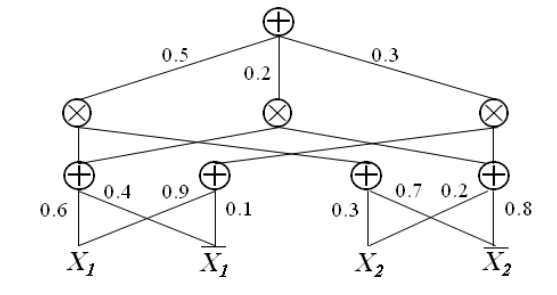
\includegraphics[scale=0.3]{graphs/spn_1.png}
    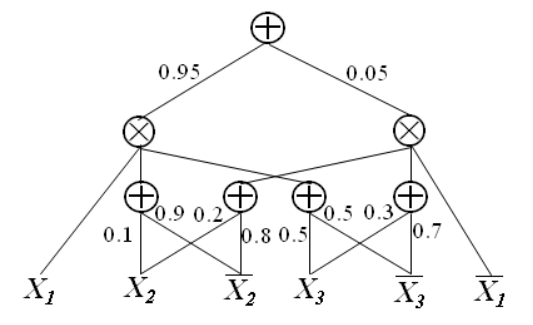
\includegraphics[scale=0.3]{graphs/spn_2.png}
    \caption{A esquerda uma SPN implementando uma naive Bayes mixture model. A direita uma SPN
    implementando uma junction tree. [P. Domingos, H. Poon]\cite{poon-domingos}}
  }
\end{figure}

\paragraph{
  Vamos assumir sem perda de generalidade que nós somas e nós produtos estão organizados de tal
  forma que somas são sempre alternadas com produtos e vice-versa. Ou seja, se $i$ é um nó soma,
  então $\forall x \in Ch(i)$, $x$ é ou um nó produto ou uma folha (e portanto uma variável).
  Analogamente, se $i$ é um nó produto, então $\forall x \in Ch(i)$, $x$ é ou um nó soma ou folha.
}

\paragraph{
  Denotamos a Sum-Product Network $S$ como uma função das variáveis indicadoras $x_1,...,x_d$ e
  $\overline{x}_1,...,\overline{x}_d$ como $S(x_1,...,x_d,\overline{x}_1,...,\overline{x}_d)$. Um
  estado $x$ é completo quando para cada variável $X_i$, seus indicadores nunca são iguais, ou
  seja, $x_i=1$ e $\overline{x}_i=0$ ou $x_i=0$ e $\overline{x}_i=1$. Se queremos $S$ em função
  de um estado $x$ completo, então representamos como $S(x)$. Se os indicadores especificam uma
  evidência\cite{project-def} $e$, então abreviamos como $S(e)$. No caso de todos os indicadores
  serem valorados em 1, então dizemos $S(*)$.
}

\paragraph{
  A subrede enraizada em um nó $n$ em uma SPN é uma SPN, e é representada como $S_n(.)$. Os valores
  de $S(x), \forall x \in \mathcal{X}$ define uma distribuição de probabilidade não-normalizada sob
  $\mathcal{X}$. A probabilidade não-normalizada da evidência $e$ é $\Phi_S(e)=\sum_{x \in e}S(x)$,
  onde a soma tem seus estados consistentes\cite{report-1} com $e$. A função partição da
  distribuição definida por $S(x)$ é $Z_S = \sum_{x \in \mathcal{X}} S(x)$. O escopo
  \cite{project-def} de uma SPN $S$ é o conjunto de variáveis que aparecem em $S$. Uma variável
  $X_i$ é negada em $S$ se $\overline{x}_i$ é uma folha de $S$ e não-negada se $x_i$ é uma folha de
  $S$.
}

\paragraph{
  A partir disso podemos construir a definição encontrada em [P. Domingos, R. Gens]
  \cite{gens-domingos}.
}

\begin{spn-def} Definimos recursivamente uma Sum-Product Network (SPN):
  \begin{enumerate}
    \item Uma distribuição monovariável tratável é uma SPN.
    \item Um produto de SPNs com escopos disjuntos é uma SPN.
    \item Uma soma ponderada de SPNs com mesmo escopo é uma SPN se todos os pesos são não-negativos.
    \item Nada mais é uma SPN.
  \end{enumerate}
\end{spn-def}

\paragraph{
  Exemplificando com a Figura 1, a SPN $S$ será:
}

\begin{equation}
  \begin{split}
    S(x_1,x_2,\overline{x}_1,\overline{x}_2)=0.5(0.6x_1 + 0.4\overline{x}_1)(0.3x_2 + 0.7
    \overline{x}_2) +\\
    + 0.2(0.6x_1 + 0.4\overline{x}_1)(0.2x_2 + 0.8\overline{x}_2) +\\
    + 0.3(0.9x_1 + 0.1\overline{x_1})(0.2x_2 + 0.8\overline{x}_2)\phantom{+}
  \end{split}
\end{equation}

\paragraph{
  E a network polynomial será a expansão de $S$, ou seja, $(0.5 \times 0.6 \times 0.3 + 0.2 \times
  0.6 \times 0.2 + 0.3 \times 0.9 \times 0.2)x_1x_2 + ...$. Se um estado completo $x = \{X_1 = 1,
  X_2 = 0\}$, então $S(x) = S(1, 0, 0, 1)$ Se a evidência $e={X_1=1}$, então $S(e)=S(1,1,0,1)$.
  E, por fim, $S(*) = S(1, 1, 1, 1)$.
}

\subsection{Propriedades}

\paragraph{
  Nesta subseção, vamos definir a validade de uma SPN, assim como completude e consistência. Em
  seguida vamos provar que uma SPN é válida se é completa e consistente. Depois vamos definir
  representabilidade, complexidade da função partição, decomponibilidade de uma SPN e finalmente
  provaremos que a função partição, probabilidade de evidência e o estado MAP\cite{report-1} de uma
  SPN podem ser computados em tempo linear no número de arestas da SPN.
}

\begin{spn-def} Uma Sum-Product Network $S$ é válida sse $S(e)=\Phi_S(e)$ para toda evidência $e$.
\end{spn-def}

\paragraph{
  A Definição 5 diz que a SPN sempre computa a probabilidade de evidência corretamente, então a SPN
  é válida. Em particular, se uma SPN $S$ é válida, então $S(*)=Z_S$. Uma SPN válida computa a
  probabilidade de evidência em tempo linear no número de arestas, como provaremos mais a frente.
}

\paragraph{
  Já que uma SPN válida é linear, é preferível aprendermos apenas SPNs válidas. Vamos ver algumas
  outras condições para a validade de uma SPN, mas para isso precisamos definir completude e
  consistência.
}

\begin{spn-def} Uma Sum-Product Network é \emph{completa} sse todos os filhos do mesmo nó soma tem
  mesmo escopo.
\end{spn-def}

\begin{spn-def} Uma Sum-Product Network é \emph{consistente} sse nenhuma variável aparece negada em
  um filho de um nó produto e não-negada em outro.
\end{spn-def}

\paragraph{
  A partir disso podemos construir o seguinte teorema de P. Domingos e H. Poon\cite{poon-domingos}.
}

\begin{spn-thm} Uma Sum-Product Network é válida se ela é completa e consistente.
\end{spn-thm}

\begin{proof}[Prova]
  $ $\newline

  Toda SPN $S$ pode ser representada por uma network polynomial $\sum_k s_k \prod_k (...)$, onde
  $\prod_k (...)$ é um monômio das variáveis indicadores e $s_k \geq 0$ é seu coeficiente (a soma
  dos produtos dos parâmetros que tenham os respectivos indicadores). Chamamos essa representação
  de \textit{expansão} da SPN, já que ela é obtida aplicando a distributiva de baixo-para-cima em
  todos os nós produtos da SPN. Ao aplicarmos a distributiva, tratamos cada folha $x_i$ como a soma
  expandida $1x_i + 0\overline{x}_i$ e $\overline{x}_i$ como $0x_i + 1\overline{x}_i$.\\

  Uma SPN é valida se sua expansão é a própria network polynomial, ou seja, se os monômios da
  expansão e os estados $x$ são correspondentes. Isso quer dizer que:

  \begin{enumerate}
    \item Cada monômio é não-zero em exatamente um estado.
    \item Cada estado tem exatamente um monômio não-zero.
  \end{enumerate}

  Pela condição 2, $S(x)$ é igual ao coeficiente $s_x$ do monômio não-zero e portanto $\Phi_s(e) =
  \sum_{x \in e} S(x) = \sum_{x \in e} s_x = \sum_k s_k n_k (e)$, onde $n_k(e)$ é o número de
  estados $x$ consistentes com $e$ que tenham $\sum_k(x)=1$.\\

  Pela condição 1, $n_k=1$ se o estado $x$ que tenha $\prod_k(x)=1$ é consistente com a evidência.
  Senão $n_k=0$ e portanto $\Phi_s(e)=\sum_{k:\prod_k(e)=1}s_k=S(e)$ e a SPN é válida.\\

  Por indução, podemos provar, começando pelas folhas até a raíz, que, se a SPN é completa e
  consistente, então sua expansão é sua network polynomial.\\

  O caso folha é trivialmente verdade, pois se o nó é folha, então ele tem apenas uma variável em
  seu escopo e portanto é completo. Pela mesma hipótese, não se pode ter uma variável negada e
  não-negada já que existe apenas um indicador, tornando-a consistente. Portanto, o caso folha é
  completo e consistente e, se computarmos sua SPN $S(l)=v_lx_l$, podemos ver que $S$ é igual a sua
  network polynomial.\\

  Consideremos agora apenas os nós internos. Assumimos apenas nós internos com dois filhos, mas a
  extensão para o caso geral é imediata. Seja $n^0$ um nó interno arbitrário com filhos $n^1$ e
  $n^2$. Teremos as seguintes notações:

  \begin{itemize}
    \item $V^i$ o escopo do nó $n^i$,
    \item $x^i$ o estado do escopo $V^i$,
    \item $S^i$ a expansão do subgrafo enraizado em $n^i$,
    \item $\Phi^i(x^i)$ a probabilidade não-normalizada de $x_i$ sob $S_i$.
  \end{itemize}

  Pela hipótese de indução, $S^1=\sum_{x^1}\Phi^1(x^1)\prod(x^1)$ e  $S^2=\sum_{x^2}\Phi^2(x^2)
  \prod(x^2)$.\\

  Se $n^0$ é um nó soma, então $S^0=w_{01}\sum_{x^1}\Phi^1(x^1)\prod(x^1)+w_{02}\sum_{x^2}\Phi^2
  (x^2)\prod(x^2)$. Se $V^1 \neq V^2$, então cada estado em $V^1$ (ou $V^2$) corresponde a múltiplos
  estados de $V^0 = V^1 \cup V^2$, e portanto cada monômio de $V^1$ (e $V^2$) é não-zero em mais de
  um estado de $V^0$, quebrando a correspondência entre monômios de $S^0$ e estados de $V^0$. Mas
  se a SPN é completa, então $V^0 = V^1 = V^2$ e seus estados são correspondentes. Portanto, pela
  indução de hipótese os monômios de $V^1$ e $V^2$ são também correspondentes e $S^0=\sum_{x^0}
  (w_{01}\Phi^1(x^0)+w_{02}\Phi^2(x^0))\prod(x^0)$, ou seja, a expansão de $S^0$ é sua network
  polynomial.\\

  Se $n^0$ é um nó produto, então $S^0=(\sum_{x^1}\Phi^1(x^1)\prod(x^1))(\sum_{x^2}\Phi^2(x^2)\prod
  (x^2))$. Se $V^1 \cap V^2 = \emptyset$, então segue-se imediatamente que a expansão de $V^0$ é a
  network polynomial. No caso mais geral, sejam $V^{12}=V^1 \cup V^2$, $V^{1--}=V^1 \setminus V^2$
  e $V^{2--}=V^2 \setminus V^1$, e sejam $x^{12}$, $x^{1--}$ e $x^{2--}$ seus estados
  correspondentes. Mas já que $\Phi^1(x^1)$ é não-zero em exatamente um estado $x^1$ e similarmente
  para $\Phi^2(x^2)$, então cada monômio no produto de $S^1$ e $S^2$ é não-zero no máximo em um
  único estado de $V^0 = V^1 \cup V^2$.\\
\end{proof}

\newpage

\printbibliography

\end{document}
